\documentclass[12pt, times new roman, a4paper]{article}
\linespread{1,5}
\usepackage[utf8]{inputenc}
\usepackage{graphicx}
\renewcommand{\figurename}{Gambar}

\begin{document}

\section{Cara Membuat Aplikasi Builder dari file Excel
ke Oracle Apex}

\subsection{ Buka aplikasi Oracle Apex Online terlebih dahulu, lalu kilk App builder}
\begin{figure}[h]
	\centering
		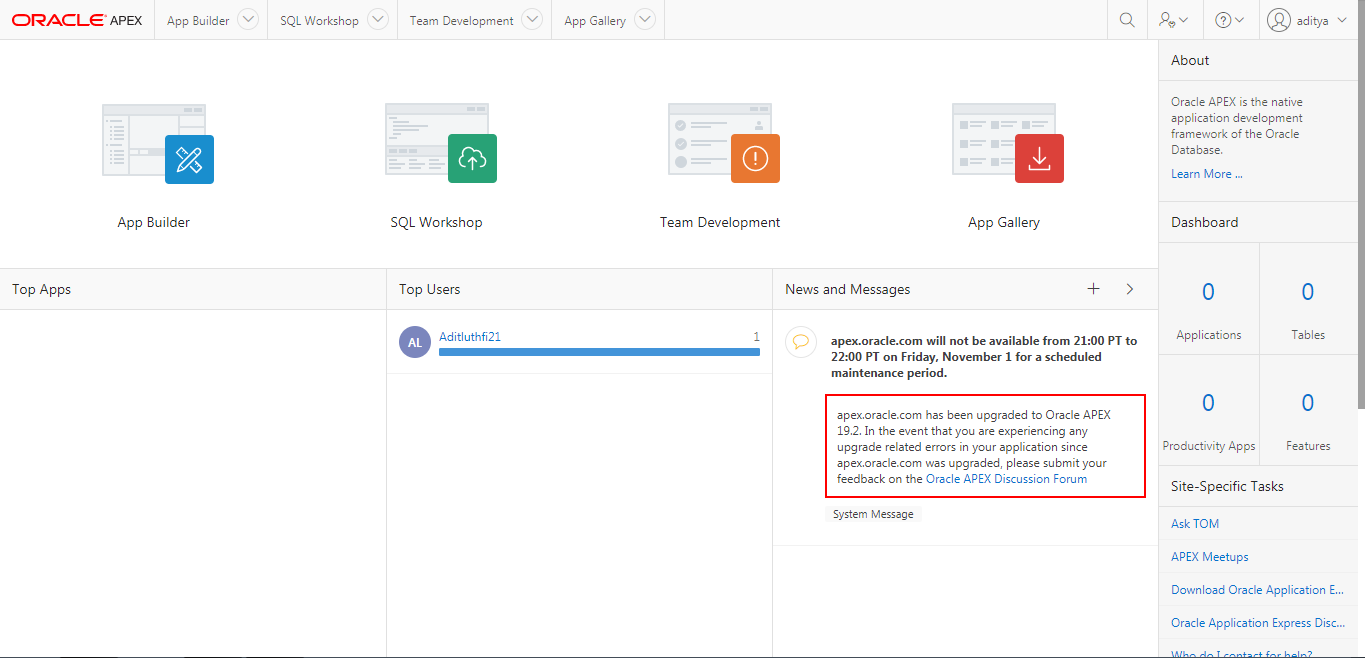
\includegraphics[scale=0.3]{gambar/1}
	\caption{Gambar Oracle APEX}
\end{figure}

\subsection{Setelah itu klik create}
\begin{figure}[h]
	\centering
		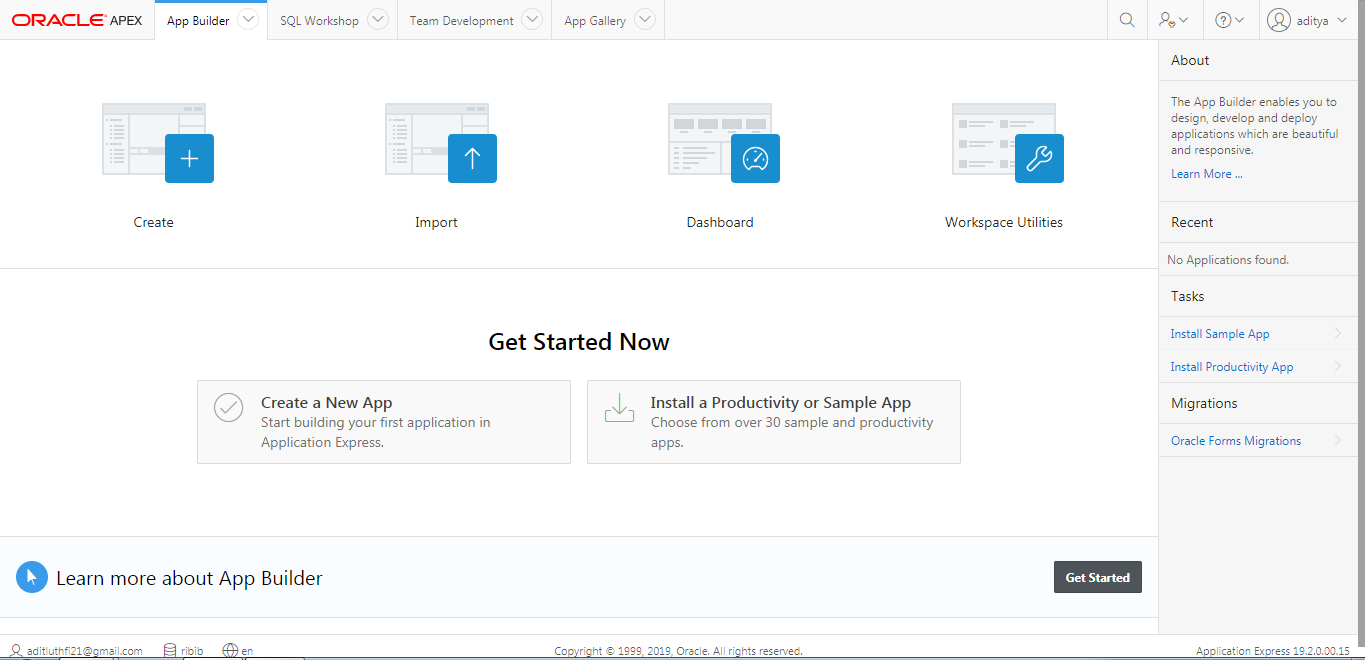
\includegraphics[scale=0.3]{gambar/2}
	\caption{Gambar Oracle APEX}
\end{figure}

\subsection{Setelah itu klik from a file}
\begin{figure}[h]
	\centering
		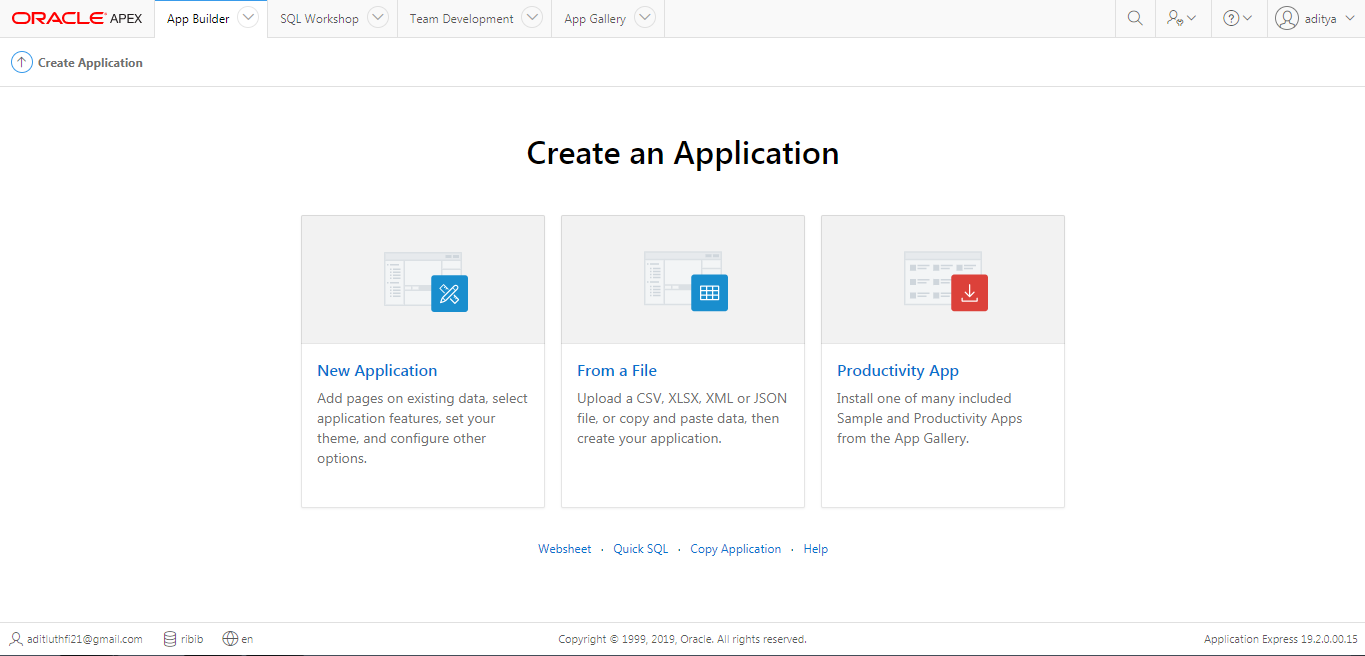
\includegraphics[scale=0.3]{gambar/3}
	\caption{Gambar Oracle APEX}
\end{figure}

\subsection{Lalu pilih file yang ingin di masukkan}
\begin{figure}[h]
	\centering
		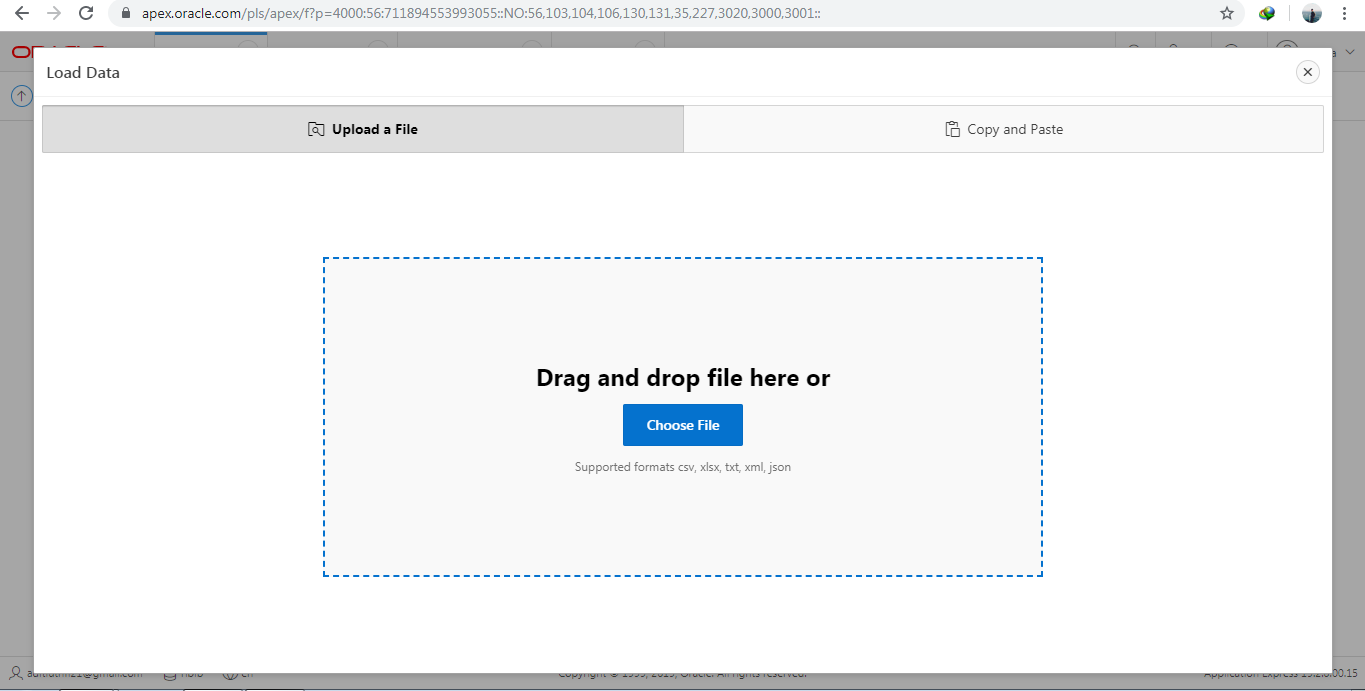
\includegraphics[scale=0.3]{gambar/4}
	\caption{Gambar Oracle APEX}
\end{figure}

\subsection{Lalu masukkan nama table}
\begin{figure}[h]
	\centering
		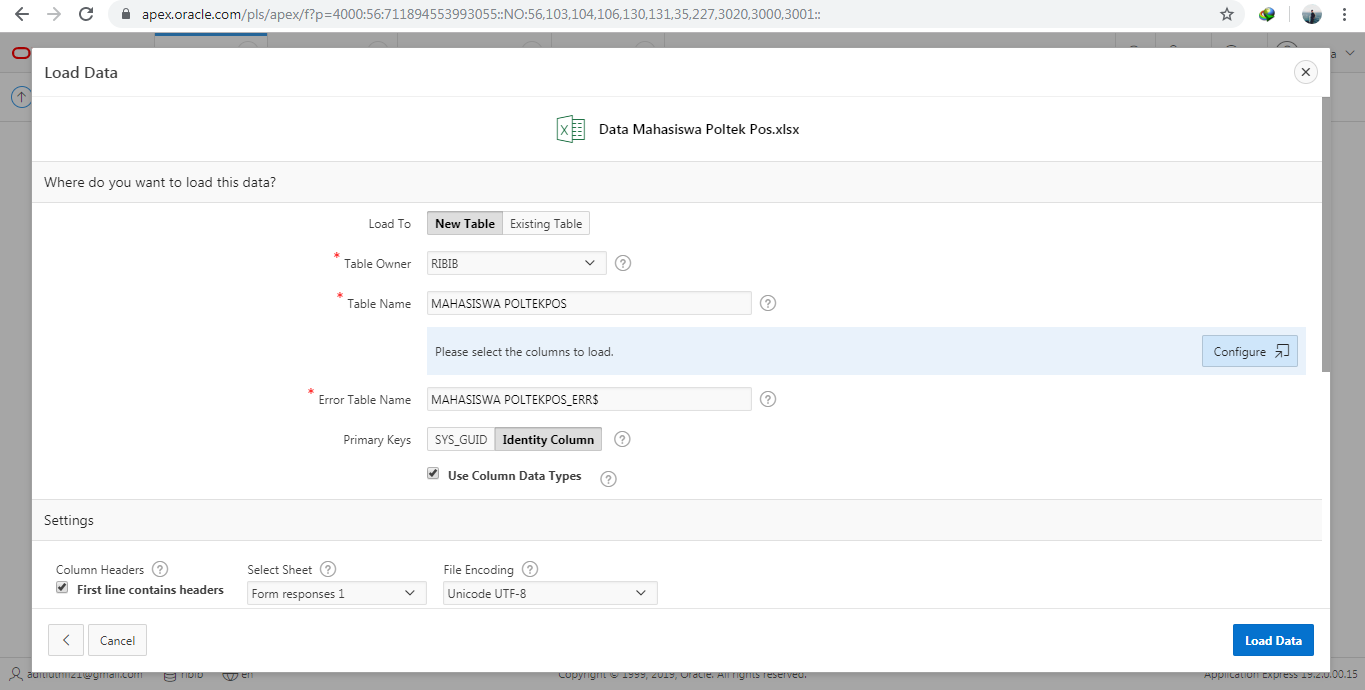
\includegraphics[scale=0.2]{gambar/5}
	\caption{Gambar Oracle APEX}
\end{figure}

\subsection{Setelah itu geser ke bawah, lalu klik preview}
\begin{figure}[h]
	\centering
		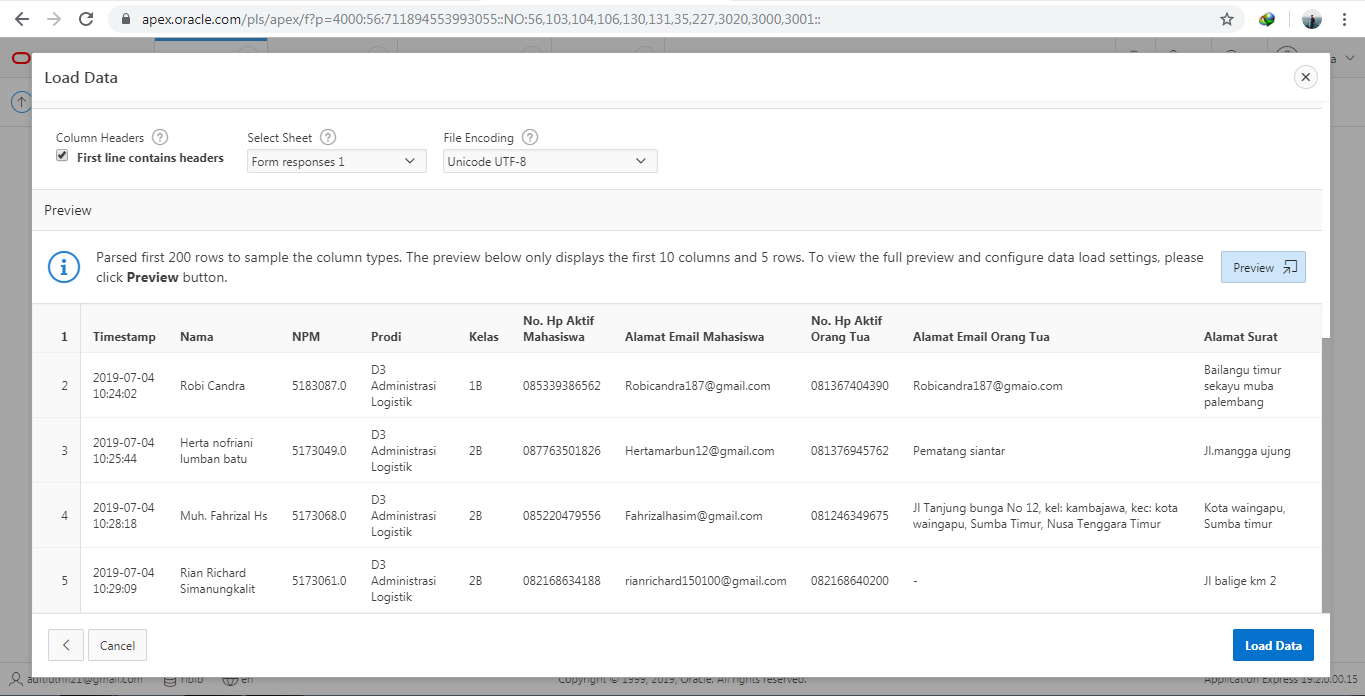
\includegraphics[scale=0.2]{gambar/6}
	\caption{Gambar Oracle APEX}
\end{figure}

\subsection{Maka data yang telah dimasukkan dapat dilihat}
\begin{figure}[h]
	\centering
		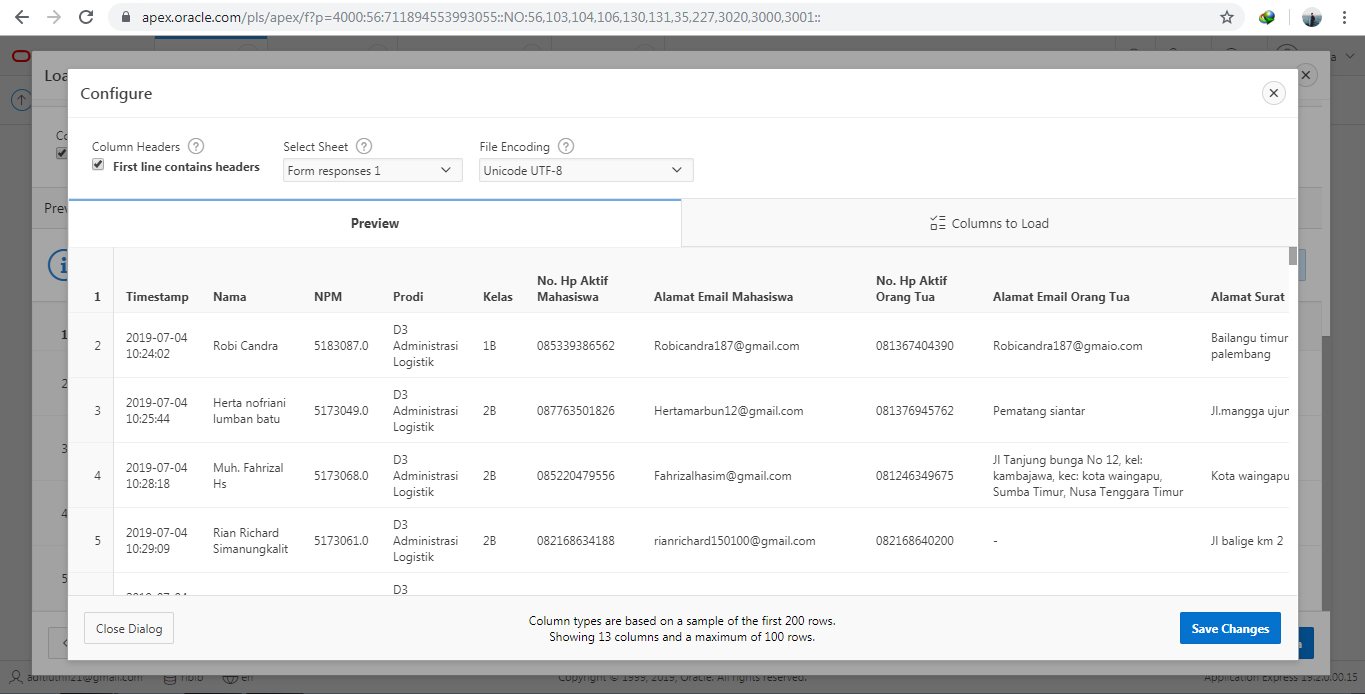
\includegraphics[scale=0.2]{gambar/7}
	\caption{Gambar Oracle APEX}
\end{figure}

\subsection{Lalu pilih create aplication}
\begin{figure}[h]
	\centering
		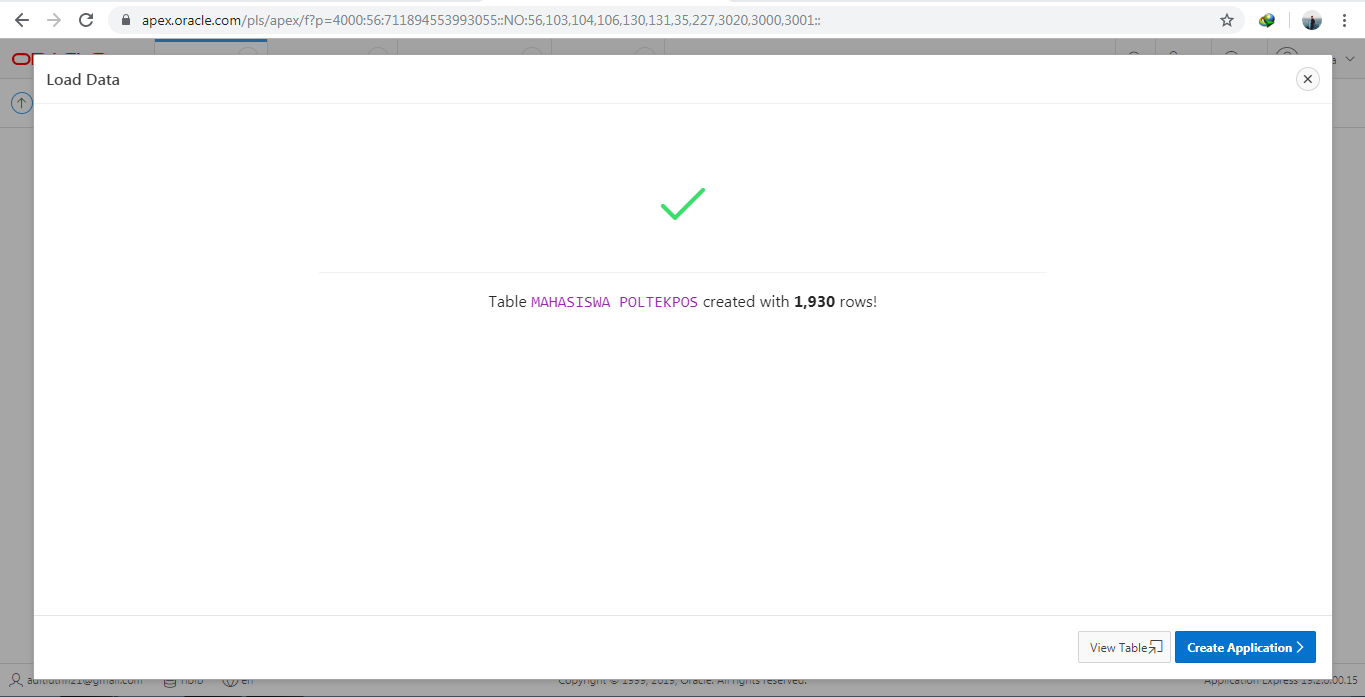
\includegraphics[scale=0.3]{gambar/8}
	\caption{Gambar Oracle APEX}
\end{figure}

\subsection{Lalu klik all pada features dan klik create application}
\begin{figure}[h]
	\centering
		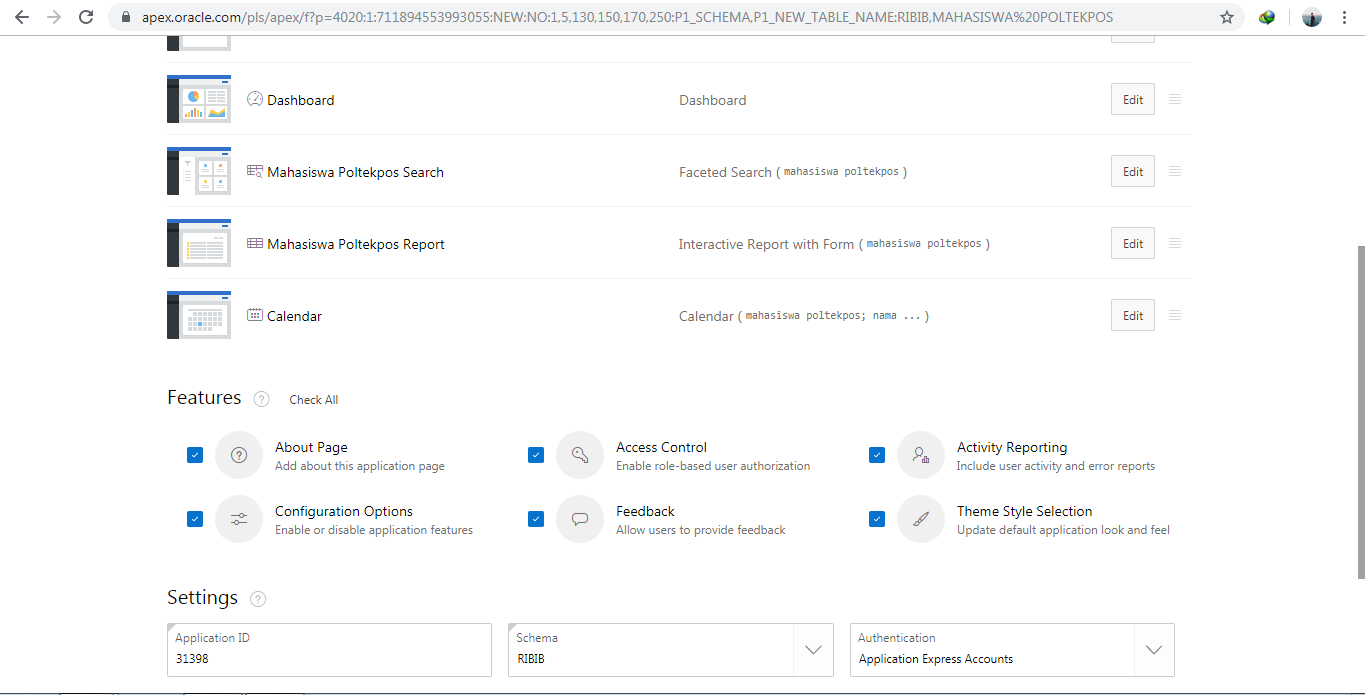
\includegraphics[scale=0.3]{gambar/9}
	\caption{Gambar Oracle APEX}
\end{figure}

\subsection{Lalu kilk run application}
\begin{figure}[h]
	\centering
		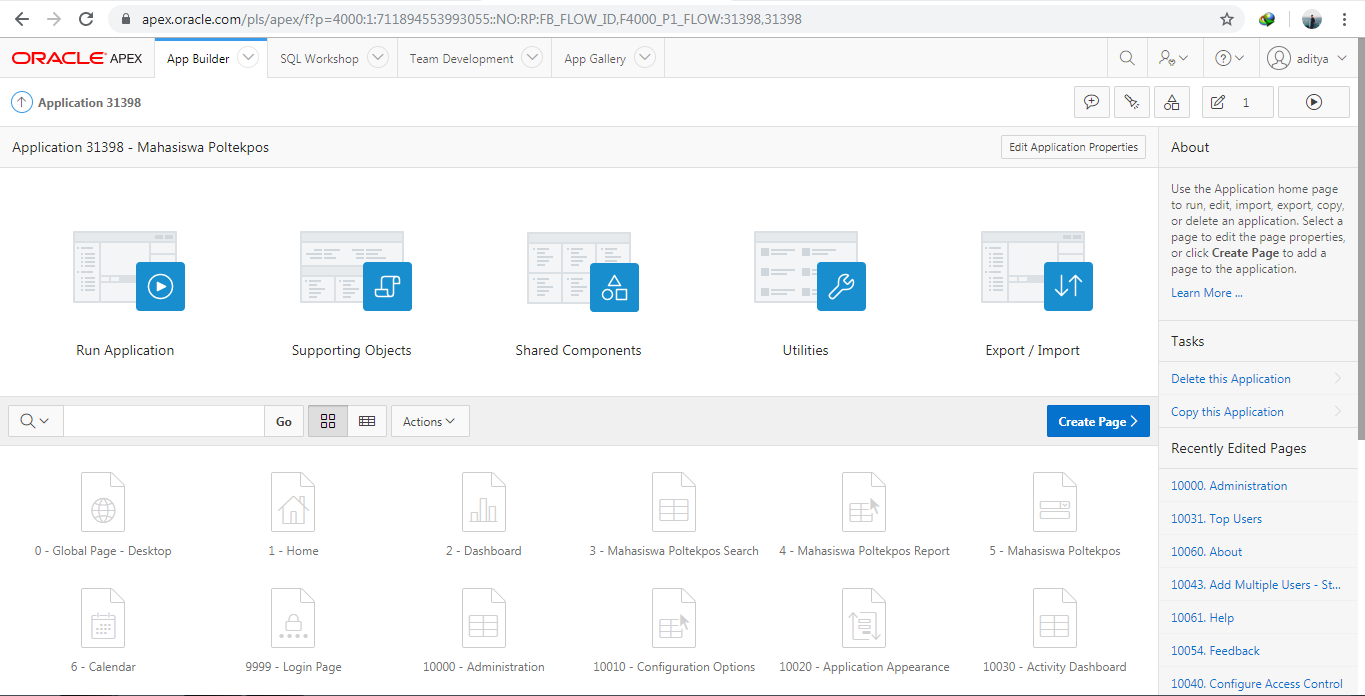
\includegraphics[scale=0.4]{gambar/10}
	\caption{Gambar Oracle APEX}
\end{figure}

\subsection{Lalu masukkan username dan password anda}
\begin{figure}[h]
	\centering
		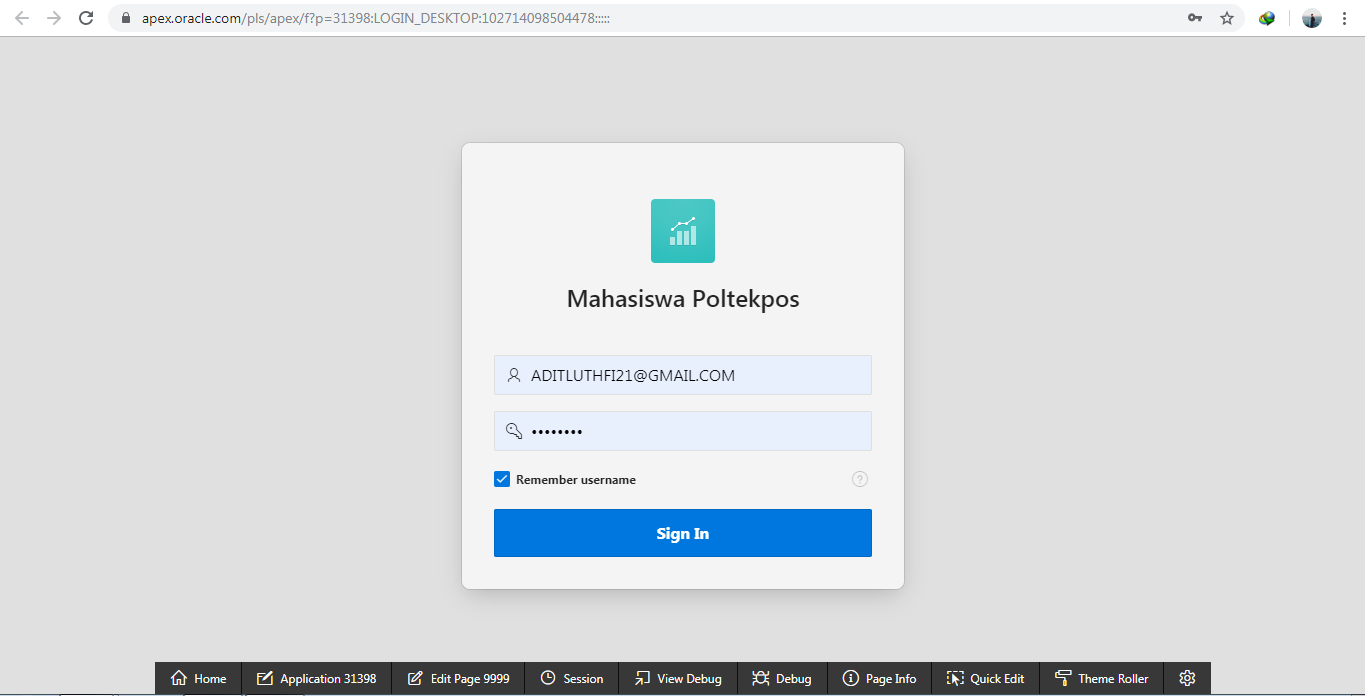
\includegraphics[scale=0.3]{gambar/11}
	\caption{Gambar Oracle APEX}
\end{figure}

\subsection{Lalu anda dapat melihat aplikasi yang sudah jadi}
\begin{figure}[h]
	\centering
		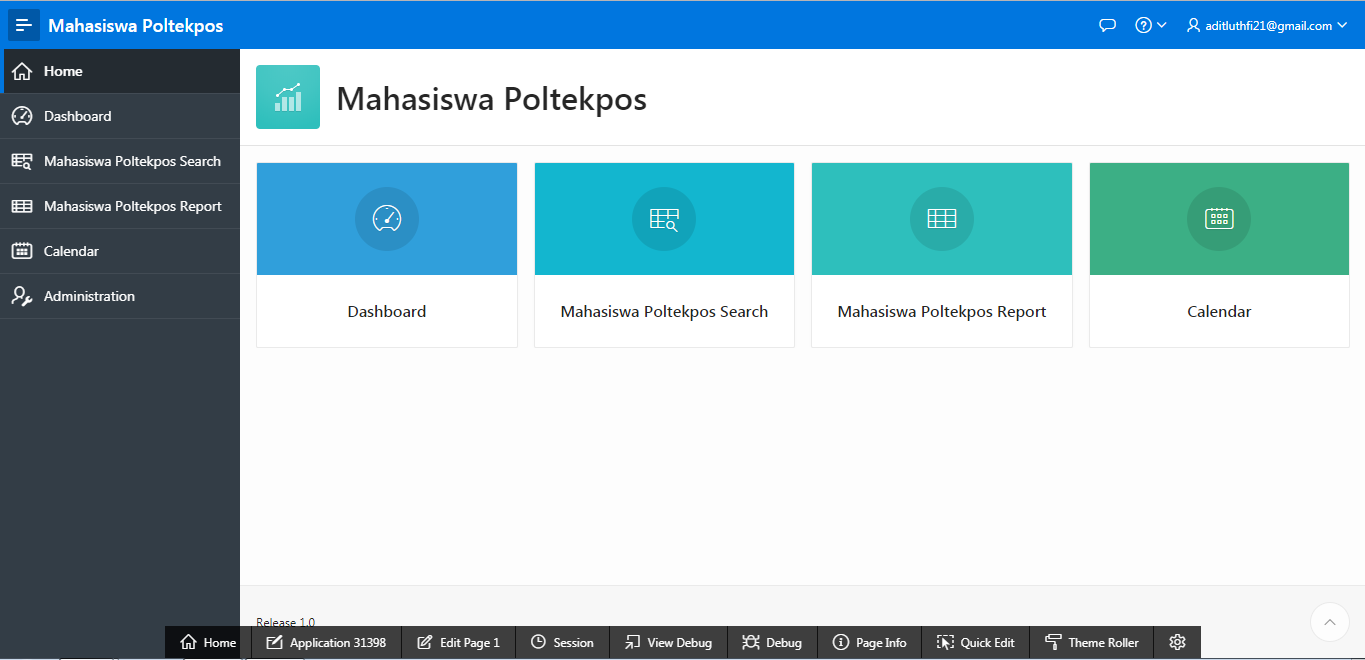
\includegraphics[scale=0.3]{gambar/12}
	\caption{Gambar Oracle APEX}
\end{figure}

\end{document}